\documentclass[12pt,a4paper]{report}

\usepackage[a4paper, margin=1in]{geometry}
\geometry{margin=1in}
\usepackage{titlesec}
\usepackage{dirtytalk}
\usepackage{graphicx}
\usepackage{amsmath}
\usepackage{hyperref}
\usepackage{setspace}
\usepackage{lmodern}
\usepackage[utf8]{inputenc}
\usepackage[T1]{fontenc}

\title{Literature Review \\ \large An Algorithmic Approach to Route Planning for Cyclists}
\author{Jack Jibb \\ MSc Computer Science}
\date{\today}

\onehalfspacing
\begin{document}

\maketitle

\tableofcontents
\newpage

\section{Training Suitability and Segmentation Algorithm Design and Analysis}

\subsection{Research Objectives}
The purpose of creating an algorithmic approach to categorizing and segmenting a GPX route is to be able to rapidly and systematically construct new routes based on the requirements of the rider's training plan.
It makes sense intuitively to segment a route, so riders does not have to analyse every part of a map to determine where to send their route. Riders are specifically interested in sections of the route such as climbs, descents, busy roads, and gravel.
The objective of research should be to come up with a suitable method of segmentation, and subsequent categorization of the resulting segments so riders can select ones that suit their training needs.
\\
Intuitively, we can segment a route by the roads that it follows, when a route changes roads, we add a segment. However this can prove more difficult to formalize, as
a road can have many intersections. How can we categorize a segment by road name but also have node values that connect to other road names that may or may not be part of the same segment?
The following research applies to the problem of Segmentation, and how we may approach defining a route segment formally.

\subsection{Algorithmic Approaches to Segmentation and Categorization}
There are several methdologies when it comes to segmentation, including (but not limited to) clustering, heuristic methods, signal analysis, and map-based segmentation. Some, or all of these may be
applied to the algorithm, since there is not one method to solve all segmentation types. What follows is a review of the literature that exists that could contribute to
achieving advanced segmentation.


\paragraph{Paul Newson and John Krumm: "Hidden Markov Map Matching Through Noise and Sparseness"}
A useful way to clean up the location data as a pre-processing step could be through map matching. Newson and Krumm \textbf{(cite here)} explore map-snapping through a HMM model on timestamp-marked latitude and longitude pairs.
The approach showcased in the paper is focused on automobile traffic, so there may be some need to tweak the emission delta for bikes, to accomodate for larger variance in the horizontal travel distance, as well as increasing
the search range for nodes around each track point. The search would then use a Gaussian probability curve, centred on GPX trackpoint, with nodes closer being more likely than ones further away. Then a transition probability will be implemented between consecutive points
so straight line distance is more probable. Lastly, a Viterbi algorithm will be run to find the "most likely" node sequence. Their approach includes two variables that need to be tweaked to maximise accuracy. This could be done via machine learning, but is out of the scope of this research. It will be set to a "good enough" setting.
Once the node sequence is determined, the sequence of ways can then be determined.


\paragraph{Wang et al., “CycleTrajectory: An End-to-End Framework for Enriching Cycling Trajectory Data”}
The authors propose a framework to provide a pipeline to correct GPS data with OpenStreetMap metadata for cycling behaviour analysis. This allows
OSM tags to be implemented into each trajectory point. This provides a fully automated and open source method for implementing OpenStreetMap data to any file that contains Latitude and Longitude points.
It also allows for a smarter noise reduction method than a simple low pass filter. Some downsides however, are that it is dependent on OSM coverage, as well as snapping errors in dense urban areas due to proximity of roads. It also relies on consistent naming and mapping schemes, when
in reality, as the data is sourced globally, not all data features will be correctly labelled or formatted.

\paragraph{Evgeny Arbatov: "GPX Route Generator"}
Arbatov provides a self-contained route planner that can take two endpoints, and plot a route between them, prioritising the shortest, but also allowing for preference, for example, preferring park-connector routes.
The application is written in Lua and is run in docker-compose. The work here provides a simple weighting mechanic, but could be useful when it comes to segmentation.
They use OSM's nearest-node API to pull intersection nodes, and generate a track from the connected ways. This means segments could be generated automatically from finding waypoints, a method for segmentation-by-road-name

\paragraph{Boeing, G: "Modeling and Analyzing Urban Networks and Amenities with OSMnx"}
Boeing Details a novel Python package that downloads and analyses street networks from OpenStreetMap, which implements simple query langauge for pulling street data from the OSM database. It also includes tools for simplifying OSM map data so
ways and nodes represent roads and intersections, which is useful for cleaning up a network created by the CyclingTrajectory framework.
As described in their Getting Started guide, the library enables a programmatic approach to visualizing OSM data as a mathematical graph. The graph
can be formatted as a GeoDataFrame, which can be exported using NetworkX and geopandas libraries. Using a function like \texttt{graph_from_bbox()}, it is possible
to obtain a road network around a geographical point, which can then return a clean and topologically correct graph $\mathcal{G}$.
It is important to note however that by reducing the map's complexity, it does increase computational complexity, so there is a trade-off there.
It can be mitigated somewhat by being a little clever about how we create a bounding box around the route.

%TODO: Implement more sources and determine a method for creating segments

\subsection{Applications in Cyclist Route Planning}
In the creation of a route, segmentation should be done automatically if a segment doesn't already exist in a database, so when a cyclist uploads their GPX file,
the route segments should be available to view.
Each route should be broken down into segments, for purpose of generating a Training Suitability Score.
A segment should be created from a series of ways, so they should always be ridable by a cyclist, and from a glance, a cyclist should be able to tell
where each segment begins and ends on a map.

\subsection{Methodological Considerations and Assumptions}
The method for segmentation via street type will be based on the factors stated in Research Objectives. In order to segment, first, each GPX file
must be separated and the data should be pre-processed. To do this, the data must be organized as such:
\begin{itemize}
	\item The GPX file must contain 1 data sample (trackpoint) per second, a rate of 1 hz.
	\item Each trackpoint must contain exactly 1 Latitude, Longitude, Elevation, and Time data point.
	\item If there is a significant gap in data ($>{}5$ seconds), the GPX file must be separated at that point.
	\item Any sudden jumps in elevation ($>{}1$ standard deviation) between two track points should be discarded
\end{itemize}
In order to maintain these requirements, the following actions may be applied:
\begin{itemize}
	\item The data may be resampled, and interpolated in order to populate data at exactly 1 hz.
	\item Interpolation may also be used to fill in missing or erroneous values due to GPS errors
\end{itemize}
There also may be some pre-calculations done to speed up processing later. These would be added to "extensions" in the GPX trackpoint.
\begin{itemize}
	\item Speed
	\item Heading (degrees from due north)
	\item Elevation Gradient (in \%)
\end{itemize}
After pre-processing, each track point (observation) will be snapped to a nearby OSM way. The map density of the road network should be considered,
since we may be able to save time with a more simplistic algorithm for snapping in areas of less route density.\\
We could also relate map density to the density of gps points, as one straight long road will need a lot fewer gps points to return a correct result than a complex series of turns.
Newson and Krumm approach this in their paper by statically removing all points that are within $2\sigma_z$ of the next point, $\sigma_z$ being the standard deviation of Gaussian GPS noise.
Their approach is specific to cars, which travel much faster than cyclists, it may be worthwhile to remove only points within $\sigma_z$ instead.kj:w

\newpage

\section{Training Suitability Scoring}

\subsection{Research Objectives}

In order to classify a segment, it is necessary to know what an athlete values in training. As a cyclist, I have used my own experience to compile this list:

\begin{itemize}
	\item Type: What is the categorization of the road? (A, B, Service, Motorway, Bike path)
	\item Surface: What is the surface of the road made of? (Tarmac, concrete, gravel, dirt, wood?)
	\item Behaviour: How does the road act? (Straight, gradual bends, sharp curves, switchbacks)
	\item Safety: How safe is this route? Are there a lot of accidents, is there a lot of commercial traffic?
	\item Elevation: Is this route a consistent gradient, is it flat, uphill, downhill, rolling?
	\item Length: How long is the route in metres.
\end{itemize}

Implementing a summative score that represents a segment will also benefit from taking rider metrics, such as Power, HR, Cadence, and Speed.
As a cyclist or group of cyclists ride a specific segment, the better picture we get of the route, as the average values will be a good representation
of the training suitability of the route.
\begin{enumerate}
	\item Safety (a composite metric defined by various factors, could also be gathered collectively from rider feedback)
	\item Difference between Average and Normalized Power (in Watts/Kg)
	\item Length (of segment)
	\item Elevation Gain (or loss)
	\item Road Quality
	\item Absolute Normal Distance Change (aka how twisty the road is)
\end{enumerate}

\subsection{Approaches to Suitability Scoring}

\paragraph{Sharifzadeh et al. "Change Detection in Time Series Data Using Wavelet Footprints"}
An interesting approach to Suitability scoring relates to Fast Fourier Transforms, and a convolution approach comes from Medhi Sharifzadeh et al, from the University of Southern California, introducing a concept known as
"wavelet footprints" as a compact, multi-resolution approach to representation of spatial-temporal trajectories. Wavelet footprints are a  more granular version of the Wavelet Transform, which in turn is a version of the Fourier Transform. The approach involves using Wavelets to transform a signal into the "Wavelet Domain".
The smaller the wavelet, the more reactive it will be to change in the original signal, so by adjusting the size of the wavelet, the signal can be filtered to be more or less reactive to change.
Wavelet footprints have an advantage over the general Wavelet transform, where they only retain the most significant components. This is done by having wavelets occur in orthoganal sets.
Due to Heisenberg's Uncertainty Principle, it is impossible to perfectly describe both the frequency content of a signal and the location in time of the signal. Time-domain and Frequency-Domain analysis in this regard are
at opposite ends of the spectrum, but the Wavelet Domain sits in the middle, allowing for a sliding scale value, where a larger scale gives more frequency and less time resolution, while smaller scales give less frequency, and more time resolution.

The advantage of using wavelet footprints over the Fourier Transform means that it is possible to isolate points in the signal where significant changes occur in specific metrics, or combination of metrics, allowing flexibility in choosing
what conditions must be met to enact a segmentation.

\paragraph{Indoor Cycling Association: "How Much Time in the Red Zone?"}
This article details a breakdown of the 7-training-zone model, which provide a good template for cutoff times for tuning Wavelet Footprints for analysing the GPX signal.
The general consensus is having 5 zones is a good compromise between continuous training definitions (specific power numbers) and binary (hard or easy). While the article describes 7 zones,
Zones 1-3 all fall outside of the hour range, which for the purpose of segment analysis would be fairly useless. The 5-Zone model approach
has good suitability to wavelet analysis, since small scale values for a wavelet would detect short burst efforts, while larger scales will detect longer, sustained effort.
Having 5 zones allows for a reduced scale array, contributing to higher performance. Here is a graphic, courtesy of the Indoor Cycling Association, that breaks down each zone. Zones 3-7 will be used for Wavelet Analysis.
\begin{figure}[h!]
	\begin{center}
		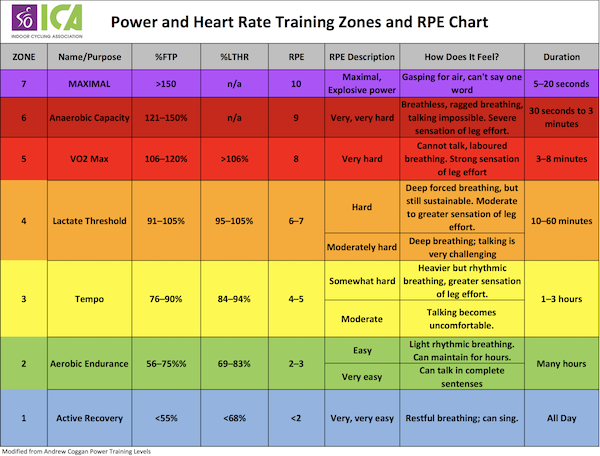
\includegraphics[width=0.6\textwidth]{zones.png}
	\end{center}
	\caption{The 7 Zone Training Model, courtesy of Indoor Cycling Association}
\end{figure}

\paragraph{Sean Hurley: "Normalized Power: What It Is and How to Use It" https://www.trainerroad.com/blog/normalized-power-what-it-is-and-how-to-use-it/}
TrainerRoad writer Sean Hurley provides a useful and consise definition of Normalized Power (NP), a metric invented by Dr. Andrew Coggan in his book \textit{Training and Racing With a Power Meter}. NP
"reflects the disproportionate metabolic cost of riding at high intensity, by weighting hard efforts and deemphasizing periods of easy spinning", according to Dr Coggan.
Essentially, NP approximates what power a rider could have put out for the same effort, if their effort was steady-state. While it is not a completely accurate metric for effort, it is a really
good indication of power variability, and as such is useful in determining the type of effort of a segment. The algorithm for determining NP is as follows:
\begin{enumerate}
	\item Calculate a rolling 30 second average power for the duration
	\item Raise each rolling average value to the fourth power.
	\item Determine the average of all the rolling values
	\item Take the fourth root.
\end{enumerate}
For an input power signal, $P(t)$ over interval $(0,N)$, the formula for Normalized Power (NP) is:
\[
	\mathrm{NP} = \bigg( \frac{1}{N} \sum_{i=1}^{N}\big(\overline{P}_{r}(i)\big)^{4}\bigg)^{1/4}
\]
where $P_r$ is the 30 second rolling average power starting at point i in the power data array.

\subsection{Applications in Training Suitability Scoring}

The application of Wavelet analysis in GPX data is a novel and flexible way of determing suitability, as it is a generic signal analysis method. Considering GPX files can
contain multiple signals, Wavelets can be applied to any discrete signal that utilizes numerical reporting. Such signals may include Power, Speed, Cadence, Heart Rate, Elevation, and Heading.
We can define wavelets of a length proportional to the maximum amount of time in training zones, as per the 5 Power Zone model, which will detect high variance up to the length. The higher the variance
at that particular training scale, the lower the suitability of the segment for that type of training.

In order to determine variance, we can use the Lipschitz Regularity to define a "variant" vs "non-variant" segment.

%TODO: Discuss Lipschitz regularity and further research and how it can be used to generate a suitability score.



\subsection{Methodological Considerations and Assumptions}
% TODO: Implement The Methodology: should have the different scoring categories, and how to obtain each one.
Power data for all methods should be first normalized, so it is not cyclist-specific. For example, power data for a professional cyclist could be an easy ride, where as for an amateur it could be an all out effort.
We have to therefore take some preliminary data points, such as rider Functional Threshold Power (FTP), and weight.
Therefore, for all power values, a power curve should be generated in advance, based on historical maximum power values for certain time thresholds.


\end{document}
